\documentclass[12 pt]{article}
\usepackage[utf8]{inputenc}
\usepackage{filecontents}
\usepackage[many]{tcolorbox}
\usepackage{graphicx}
\usepackage{harpoon}
%\usepackage{apacite} 
\usepackage{xcolor}
\usepackage{latexsym}
\usepackage{amssymb}
\usepackage{amsmath}
\usepackage{mdframed}
%\usepackage[authoryear]{natbib}
\usepackage{hyperref, url}
\usepackage[show]{ed}
\usepackage{subfigure}
\usepackage[ntheorem]{empheq} 
\usepackage{amsthm, amssymb, amsfonts, latexsym}
\usepackage{pst-all}

\usepackage{enumitem}

\setlength{\parskip}{1.7em}
\setlength{\parindent}{0em}


%\setlength{\baselineskip}{20pt}

\setlength{\textwidth}{429.75499pt}
\setlength{\textheight}{643.20255pt}
\setlength{\oddsidemargin}{5 mm}
\setlength{\evensidemargin}{5 mm}
\setlength{\topmargin}{0 mm}
\setlength{\headsep}{0 mm}
\setlength{\headheight}{0 mm}



\newcommand{\citealtt}[1]{\citeauthor{#1},\citeyear{#1}}
\newcommand{\myycite}[1]{\citep{#1}}

\mathchardef\mhyphen="2D

%\newcommand{\cev}[1]{\reflectbox{\ensuremath{\vec{\reflectbox{\ensuremath{#1}}}}}}


\usepackage{pst-node,graphicx,pst-blur}
%\uspackage{auto-pst-pdf}
%\usepackage{tikz-cd} 



\makeatletter
\DeclareRobustCommand{\cev}[1]{%
  \mathpalette\do@cev{#1}%
}
\newcommand{\do@cev}[2]{%
  \fix@cev{#1}{+}%
  \reflectbox{$\m@th#1\vec{\reflectbox{$\fix@cev{#1}{-}\m@th#1#2\fix@cev{#1}{+}$}}$}%
  \fix@cev{#1}{-}%
}
\newcommand{\fix@cev}[2]{%
  \ifx#1\displaystyle
    \mkern#20mu
  \else
    \ifx#1\textstyle
      \mkern#20mu
    \else
      \ifx#1\scriptstyle
        \mkern#26mu
      \else
        \mkern#26mu
      \fi
    \fi
  \fi
}

\makeatother

\newcommand{\xcm}{\epsfxsize=3.1cm}
\newcommand{\fig}[1]{\epsfbox}
% \newcommand{\bp}{\begin{minipage}{3.1cm}}
% \newcommand{\ep}{\end{minipage}}



\newtheorem{Definition}{Definition}[]
%\newmdtheoremenv{Theorem}{Theorem}[]
\newtheorem{Theorem}{Theorem}[]
\newtheorem{Lemma}{Lemma}[]
\newtheorem{Proposition}{Proposition}[]
\newtheorem{Corollary}{Corollary}[]
\newtheorem{Remark}{Remark}[]
\newtheorem{Example}{Example}[]




\makeatletter 
\renewcommand{\thefigure}{\@arabic\c@figure}
\makeatother
\usepackage{xr}


%%%% PNAS GRAPHICS SETUP- FROM THE PNAS STYLE LATEX FILE
\RequirePackage{graphicx,xcolor}
\RequirePackage{colortbl}
\RequirePackage{booktabs}
\RequirePackage{algorithm}
\RequirePackage[noend]{algpseudocode}
\RequirePackage{changepage}
\RequirePackage[twoside,%
				letterpaper,includeheadfoot,%
				layoutsize={8.125in,10.875in},%
                layouthoffset=0.1875in,%
                layoutvoffset=0.0625in,%
                left=38.5pt,%
                right=43pt,%
                top=43pt,% 10pt provided by headsep
                bottom=32pt,%
                headheight=0pt,% No Header
                headsep=10pt,%
                footskip=25pt,
                marginparwidth=38pt]{geometry}
\RequirePackage[labelfont={bf,sf},%
                labelsep=period,%
                figurename=Fig. ]{caption}
\setlength{\columnsep}{13.5pt} % Distance between the two columns of text
\setlength{\parindent}{12pt} % Paragraph indent

%% Figure caption style
\DeclareCaptionFormat{pnasformat}{\normalfont\sffamily\fontsize{7}{9}\selectfont#1#2#3}
\captionsetup*{format=pnasformat}

%%% GREYBOX AROUND FIG
\definecolor{lightgray}{gray}{0.95}
\newcommand\greybox[1]{%
  \vskip\baselineskip%
  \par\noindent\colorbox{lightgray}{%
    \begin{minipage}{\textwidth}#1\end{minipage}%
  }%
  \vskip\baselineskip%
}

\newtcolorbox{paperbox}[1][]{
    enhanced,
    colback=white,
    boxrule=0pt,
    boxsep=0pt,
    arc=0mm,
    width=0.8\linewidth,
    fuzzy shadow={0mm}{-4pt}{-4pt}{1mm}{black!30!white},
    #1
}


\externaldocument{Supp_Koopman-0808}
\begin{document}



\title{Project Thesis/Report}



\author{} 
\date{}
\date{}
\maketitle

\section{Introduction}

Experimenting on biological, physical, and artificial systems in order to generate a more informative dynamical model is a well-established practice in modern science. Traditional methods for modelling physical systems are based on laws of physics that are based either on empirical relationships or on intuition. For systems that evolve with time, physical laws yield mathematical equations that govern how the quantities evolve with time. However our world around is, for the most part, much more complex than that which can be distilled into elegant equations. We do not fully understand many of the more complex systems, nor do they even provide us with a good physical intuition of the underlying principles governing the dynamics.

To complicate this - the underlying systems we observe often display sensitive dependence on initial conditions; despite having highly similar initial conditions, differing orbits diverge quickly and to such an extent that it becomes seemingly impossible to retrace their steps back to the original conditions. Even the presence of usually 'negligible' computational noise or measurement error renders long-term point-wise prediction infeasible. 
There are many difficulties that one encounters while modelling such systems:
\vspace{-8mm}
\begin{enumerate}[noitemsep, label=\roman*.]
  \item One may not have access to the complete states of the systems
  \item The actual system may be described by functions that behave wildly in the sense their graphs have a wild oscillatory behaviour, i.e., they have a large functional complexity.    
\end{enumerate}


Models derived primarily from data can be classified into three categories: 
\vspace{-8mm}
\begin{enumerate}[noitemsep, label=\roman*.]
  \item  Interpretable models (i.e., they establish relationships between internal physical mechanisms), 
  \item Partially interpretable models capturing some modes of the dynamics, 
  \item Non-Interpretable models, defined as such mainly due to the fact that they are defined on a different phase space that is usually high-dimensional. 
\end{enumerate}

Examples in the literature attempting to forecast data from such systems have tried a number of different approaches with differing degrees of success. One could learn a system conjugate to the underlying system by applying the Takens delay embedding; this learnt system could then be used for forecasting the original system. \cite{takens1981detecting}. An ordinary differential equation can be obtained from data (Citations to Sindy). Alternatively, one could approximate the vector field by a library of functions (Citations to Sindy) to obtain interpretable models. Takens delay methods suffer from lack of robustness to noise and may not yield a learnable map that has lower functional complexity (See Section 3). For the methods that build interpretable models (Citations to Sindy) the complete system states are needed which is rarely available. Pure machine learning methodology that processes temporal information (like the echo state networks (Citations to echo state networks)) is an approach that maps data onto a higher dimensional space for further processing. Although they perform  well on forecasting some dynamical systems, they fail completely on others (Citations here) as there is often guarantee that the right function was learnt during training.

Recent partially interpretable models available in the literature have been based on the Koopman operator (e.g.,\cite{koopman1932dynamical,budivsic2012applied}) to  employ observables mapping the data onto a higher-dimensional space. This then makes the dynamics in the higher-dimensional space more amenable for approximation by a linear transformation. Such methods, obviously, do not guarantee an exact reconstructions for nonlinear models, and in practice provide poor long-term consistency for a large class of systems. (Add citation)

The non-interpretable models include the delay embedding and the machine learning algorithms. Under some generic conditions, the Takens delay embedding theorem \cite{takens1981detecting} and its various generalisations (e.g., \cite{sauer1991embedology, stark1999delay, gutman2018embedding, gutman2018embedding}) establishes the learnability of a system constructed by concatenating sufficiently large previous time-series observations of a dynamical system into a vector (called delay coordinates). This then establishes the existence of a map on the space of delay coordinates equivalent (or topologically conjugate) to the underlying map from which the observed time-series was first obtained. Although topological conjugacy guarantees an alternate representation of the underlying system, the quality of thsi representationstill depends on numerous parameters, making the comprehension of the dynamics rather unreliable (e.g., \cite{principe1992prediction}). One reason for this fragility is that the embedded attractor in the reconstruction space not always an attractor itself, despite  unquestionably being an invariant set. Since the embedded object is not \emph{(definitely/always?)} an attractor (as explained in Chapter 3) it can cause predictions to fail.


Practically, the application of Takens embedding involves learning a map through some technique and consequently one wishes that these would have low functional complexity\cite{manjunath2021universal}, i.e., functions with fewer oscillatory graphs.

This thesis deals with the implementation and analysis of non-interpretable models that can guarantee \emph{exact/accurate} reconstruction. The project work concerns the study and implementation of a method (Citation to paper with Adriaan) that incorporates learning a function by mapping the data on to a higher dimensional space. With a clear understanding of how the data is mapped onto the higher dimensional space, the method then permits the learning of a dynamical system topologically conjugate to that of the underlying system. Instead of linear regression, deep learning methods are employed to learn the correct function. With slight modifications to the implementation in the paper (with Adriaan), we show that one can construct accurate non-interpretable models with the ability to reconstruct attractors from more hard-to-forecast systems like the double pendulum. (The forecasting of the time-series from a double pendulum has not been reported before.) Moreover, we also demonstrate that long-term statistical consistency is preserved.

By solidifying the mathematical underpinnings of our theory, we hope to guarantee the ability to construct models with predictive power ranging from molecular biology to neuroscience. in the near future. (We can modify this sentence when the report is completed.)

The report is organised as follows: 
\newline In Section 2, we recall the definition of a discrete-time dynamical system, how a discrete-system arises from a flow of an ODE and then proceed to define the inverse limit space and topological conjugacy of autonomous systems. 
\newline In Section 3, we introduce the problem of forecasting dynamical systems, state the Takens delay embedding theorem and discuss various issues faced while forecasting. 
\newline In Section 4, a driven dynamical system is defined and discuss the properties of a specific class of driven dynamical systems that we make use of in this theses/report/paper. 
\newline Finally in Section 5 we show the implementation of these forecasting methods, and conclusions are provided in Section 6.


\section{Discrete-time Dynamical Systems}

In this chapter, we provide a brief description of what a discrete-time dynamical system is and what it means for it to exhibit chaos. We refer to \cite{devaney2018introduction, de2013elements} for more details. 

At its most elementary level, a dynamical system is just \emph{something} that evolves deterministically through time. In the context of this thesis, deterministic refers to the fact that a system evolves according to specified rules rather than based on random events. 
Dynamical systems arise in a variety of situations. A continuous dynamical system, and here specifically the motion of a pendulum, is one in which quantities such as the angular position and angular momentum are known at all times. 
The equations of the dynamical system take the form of one or more ordinary differential equation that determine the relevant quantities at any future time if we know the initial location and momentum. 
In ecology, discrete dynamical systems are widely used to model population growth. The model in this case is a function calculating the following generation's population given the population of the previous generation. If we know the starting population, we may once again calculate the population at any time in the future. 

Formally, a function $T: U \to U$, where $U$ is some set is  a \emph{discrete-time dynamical system} and its iterates $\{u,Tu,T^2u,\ldots\}$, where $T^n$ denotes the $n$-fold composition of $T$ with itself, describe the evolution of an initial condition $u\in U$ (Note that we drop the brackets and denote $T(u)$ by $Tu$ for simplicity).  





Continuous dynamical systems modelled using ordinary differential equations can give rise to discrete-time dynamical systems. To see this, consider differential equation $\dot{x} = f(x)$, $f: \mathbb{R}^n \to \mathbb{R}^n$, $n\in\mathbb{N}$ given to have a unique solution passing through 
each point $x\in\mathbb{R}^{n}$, the \emph{flow of the equation} is defined to be a mapping $\varphi: \mathbb{R}^n \times \mathbb{R} \to \mathbb{R}$ that satisfies the following properties:
\vspace{-8mm}
\begin{enumerate}[noitemsep, label=\roman*.]
  \item $x(t)$ is a solution of the differential equation,
  \item $x(0)=x_0$, and
  \item $\varphi(x_0,t) = x(t)$.
\end{enumerate}
By fixing $t=K$, we can define the \emph{time-$K$ map} as  $T(x):= \varphi(x_0,K)$, and it is easily verified that $T\circ T(x_0) = \varphi(x_0,2K)$. In general the $m^{th}$ iterate of $x_0$ under $T$ would be the value of the solution of the ODE evaluated at time $mK$ with the initial condition $x_0$. 
Thus ordinary differential equations give rise to a discrete-time dynamical systems by sampling the value of $x$ at time intervals $K$ units apart. 

Of course, discrete-time dynamical systems need not always arise through a differential equation, and once again we may consider the field of ecology where discrete dynamical systems are often directly derived or assumed. 
\emph{There is a school of thought that advocates discrete-time dynamical systems to be more natural for modelling real-world observations than differential equations (see \cite{saber2010introduction}).  <- too philosphical, or actually good?}

A numerical discretization of a differential equation can also give rise to a discrete-time dynamical system. For instance, Euler's method approximates $\dot{x}(t)$ by $(x(t+h)-x(t))/h$; if $h$ is fixed throughout, the solution of a differential equation $\dot{x}=f(x)$ 
can be approximated at the time instant $t+(m+1)h$ by iterating the equation 
$$x(t+(m+1)h) = x(t+mh) + h f(x(t+mh)).$$ 
Adopting more succinct notation by replacing $x(t+mh)$ with $u_m$, we rewrite the above equation as
$$u_{m+1} = u_m + hf(u_m)$$
or, in even simpler terms, as the discrete-time dynamical system with map $T(u) = u + hf(u)$, where $T$, $u$ and $f$ are understood to be as above.

\subsection{Invariant Sets}

A core concept in the study of dynamical systems is that of invariance. Given a discrete-time dynamical system $T: U \to U$, a subset $A \subset U$ is said to be an \emph{invariant set} if $T(A) =A$. 
We also define the \emph{orbit of T} to be a sequence $\bar{u} = \{u_n\}_{n\in \mathbb{Z}}$ obeying the update equation, $u_{n+1}=Tu_n$, $n \in \mathbb{Z}$. 


Two examples of invariant sets include a fixed point where $Tu=u$ for  $u\in U$, and a periodic orbit, i.e., a set of iterates $\{u,Tu, T^2u,\ldots,T^pu\}$, where $T^{p+1}u=u$ for some $p$.  The entire space $U$ could be also be invariant.
Consider for example the space $U=[0,1]$, where $Tu=4u(1-u)$ and then $U$ is invariant. \emph{(as every $u\in{U}$ can be written as $u = 4x(1-x)$ for some $x\in{U}$)}

We may learn a great deal about the iterates of a dynamical system by considering the types of invariant sets of a discrete-time dynamical system.  For example, if $U=[0,1]$ has map $Tu= u/2$, then the only invariant set is $\{0\}$, and all orbits approach this invariant set as time flows in the forward direction. 
Indeed, if a some non-zero invariant set (call it $B$) exists, then there is  some $r\in(0,1]\cap{B}$. But $r\notin{T(B)}$ since any orbit with initial value $r$ will be a decreasing sequence. Moreover, every orbit of T will be decreasing and therefore approach the value $0$ as $n\rightarrow\infty$

One may ask if every orbit approaches an invariant set? In general the answer is no, since for the dynamical system $Tu=2u$, any orbit that does not intersect the invariant set $\{0\}$, will not approach any invariant set. 

However,  when the space $U$ is compact, all orbits approach an invariant set. \textbf{For let $\bar{u} = \{u_n\}_{n\in \mathbb{Z}}$ be an orbit in the compact space U, then $\bar{u}$ has a convergent subsequence }

\textbf{In fact the $\omega$-limit set $\omega(u;T)$ of a point $u$ defined to the collection of limit points of the sequence $\{x,Tu,T^2u,\ldots\}$ is nonempty, and $\omega(u;T)$ is invariant. } (not relevant other than being an additional example perhaps?)

We discuss various properties of invariant sets: Invariant sets can be attracting or repelling depending on how orbits in its vicinity behave (recall the examples $Tu =u/2$ and $Tu=2u$). We are interested in attractive invariant sets, and in particular so-called attractors which we define below.
\begin{Definition} \rm Let $T: U \to U$, where $U$  is a metric space with metric $d$. A compact subset $A \subset U$ is said to be an attractor if it satisfies the three conditions: 
  \vspace{-8mm}
  \begin{enumerate}
	\item $A$ is invariant. 
	\item $A$ is asymptotically stable, i.e., for every $\epsilon > 0$ and for all $u$ so that $d(u,A) < \epsilon$, we have $d(T^nu,A) \to 0$ as $n\to \infty$. 
	\item $A$ has Lyapunov stability, i.e., for every $\epsilon > 0$  there exists a $\delta(\epsilon) > 0$ so that $d(u,A) < \delta$ implies $d(T^nu,A) < \epsilon$ for all $n\ge 0$.  
\end{enumerate}
\end{Definition} 

In our previous examples, the system  $Tu=u/2$ had the singleton set $\{0\}$ as an attractor. For the system,  $Tu=4u(1-u)$ on $[0,1]$, one may easily verify that the only attractor is the entire space $[0,1]$. \textbf{For let $B$ be an attractor of U. From above, we know that B is itself invariant, is asymptotically stable and has Lyapunov stability. Now suppose there is some attractor $C\subsetneq{U}=B$, so there is a $b\in{U}$ which is not in $C$. ........  }

A dynamical system can have several attractors, and may also be contained in another attractor. 

% If the dynamics on the attractor are somewhat complicated in the sense that the attractor cannot be decomposed further, and if the attractor is infinite then there is a possibility of complicated dynamics, and a particular well-studied phenomenon of such complexity gives rise to what is called a chaotic behaviour. 

If the dynamics on an attractor cannot be decomposed further and the attractor is itself also infinite, then there is a possibility of complicated dynamics, and a particular well-studied phenomenon of such complexity gives rise to what is called chaotic behaviour. 

\subsection{Chaos}

\emph{$\downarrow$ - should one add paragraphs like these?}
\newline In the 1960s, a number of mathematicians and mathematically interested scientists independently discovered chaos in the mathematical sense. The meteorologist Edward Lorenz may have been the first to explain this phenomenon in his 1963 paper \cite{lorenz1963deterministic}. The notions of invariance, attractivity and chaos may also bedescribed for continuous systems, and Lorenz's system comprised of a system of differential equations. The narrative of Lorenz's discovery of chaos, as well as the history of other forerunners in this subject, are fascinating. For those who are interested, we highly recommend James Gleick's book Chaos: The Making of a New Science \cite{gleick2008chaos}. It clearly illustrates these experiences, explains why chaos was such a startling and crucial mathematical and scientific discovery, and describes the underlying mathematical notions for non-specialists.

There are several intricately different notions of chaos, with each of them indicating some complexity. \emph{ $\leftarrow  $ what are we saying here?} In practice, it is not possible to verify which notion is satisfied when data is observed from a dynamical system. We do, however, specifically recall the definition of chaos in the sense of Devaney \cite{devaney2018introduction,de2013elements} so as to understand some nuances. Devaney's definition consists of three parts, with the first being the notion  of sensitive dependence on initial conditions. 

\begin{Definition} \rm 
A dynamical system $T: U \to U$ is said to have sensitive dependence on initial conditions (SDIC) if there exists a $\delta > 0$ such that for every $u \in U$ and in every neighborhood of $u \in U$ there exists a $v\in{U}$ and an integer $N:=N{(u,v)}\in\mathbb{Z}$ such that $d(T^Nu,T^Nv)>\delta$. 	
\end{Definition}

It is important to acquire a sense of this definition as it can easily be misunderstood. It is common misconception to interpret SDIC as two close points ($u$ and $v$) that eventually become separated by a distance $\delta$ under iteration by $T$. But this is not true. To fully comprehend all the subtleties of the concept, one needs to discuss it more thoroughly by considering each sentence with care and attention, whereafter one may examine how they fit together to convey the concept of sensitive dependence. \emph{ $\leftarrow$ is this talking too simply perhaps?}. 

To this end we make 3 remarks:
\vspace{-5mm}
\begin{enumerate}
  \item First, the $\delta>0$ in the definition of SDIC is independent of $u$. 
  \item Second, in every neighborhood of $u$, we may not necessarily find all points $v$ in the neighborhood distinct from $u$ that would separate from the forward iterates of $u$. 
  \item  Finally, $N$ depends upon $u$ and $v$ chosen, and their iterates may not separate for ever (i.e., for all $n>N$) and we allow their iterates to get arbitrarily close in the future. 
\end{enumerate}


 
\ednote{M: It is probably best to see a few numerical simulations to understand SDIC. (Please use the logistic map and perhaps the trajectories of the double pendulum data). } 

The second part in Devaney's definition of chaos concerns topological transitivity.

\begin{Definition}
	A dynamical system $F: U \to U$ is topologically transitive if for any pair of nonempty open sets $E_1$ and $E_2$ there exists a $n\in\mathbb{N}$ such that $T^n(E_1) \cap E_2 \not= \emptyset$. 
\end{Definition}

Topologically transitivity implies that the iterates of an open set of initial conditions gets mixed up with other open sets. On a compact metric space, it can be shown that topological transitivity also implies the existence of a point whose forward iterates are dense; or in other words, the orbit going through this point will be dense in the compact metric space. 

In fact, it is topologically more likely that the choice of an arbitrary point will be one  whose iterates are almost dense.
% I inserted a definition here: it makes more sense to me. 
\begin{Definition}
A compact metric space $U$ is said to be almost dense if the complement of the set of points which are dense in $U$ may be written as a countable union of sets of with empty interior. In other words, the set on points not dense on $U$ is topologically insignificant.
\end{Definition}

We may now define the notion of Chaos as formulated by Devaney\cite{devaney2018introduction}.
\begin{Definition}
	A dynamical system $T: U \to U$ is said to exhibit chaos in the sense of Devaney if it satisfies the three properties:
	\vspace{-5mm}
  \begin{enumerate}
		\item $T$ has SDIC.
		\item $T$ is topologically transitive.
		\item The set of periodic points of $T$ are dense in $U$. 
	\end{enumerate}
\end{Definition}


\begin{figure}
  \centering
  \begin{minipage}{.5\textwidth}
    \centering
    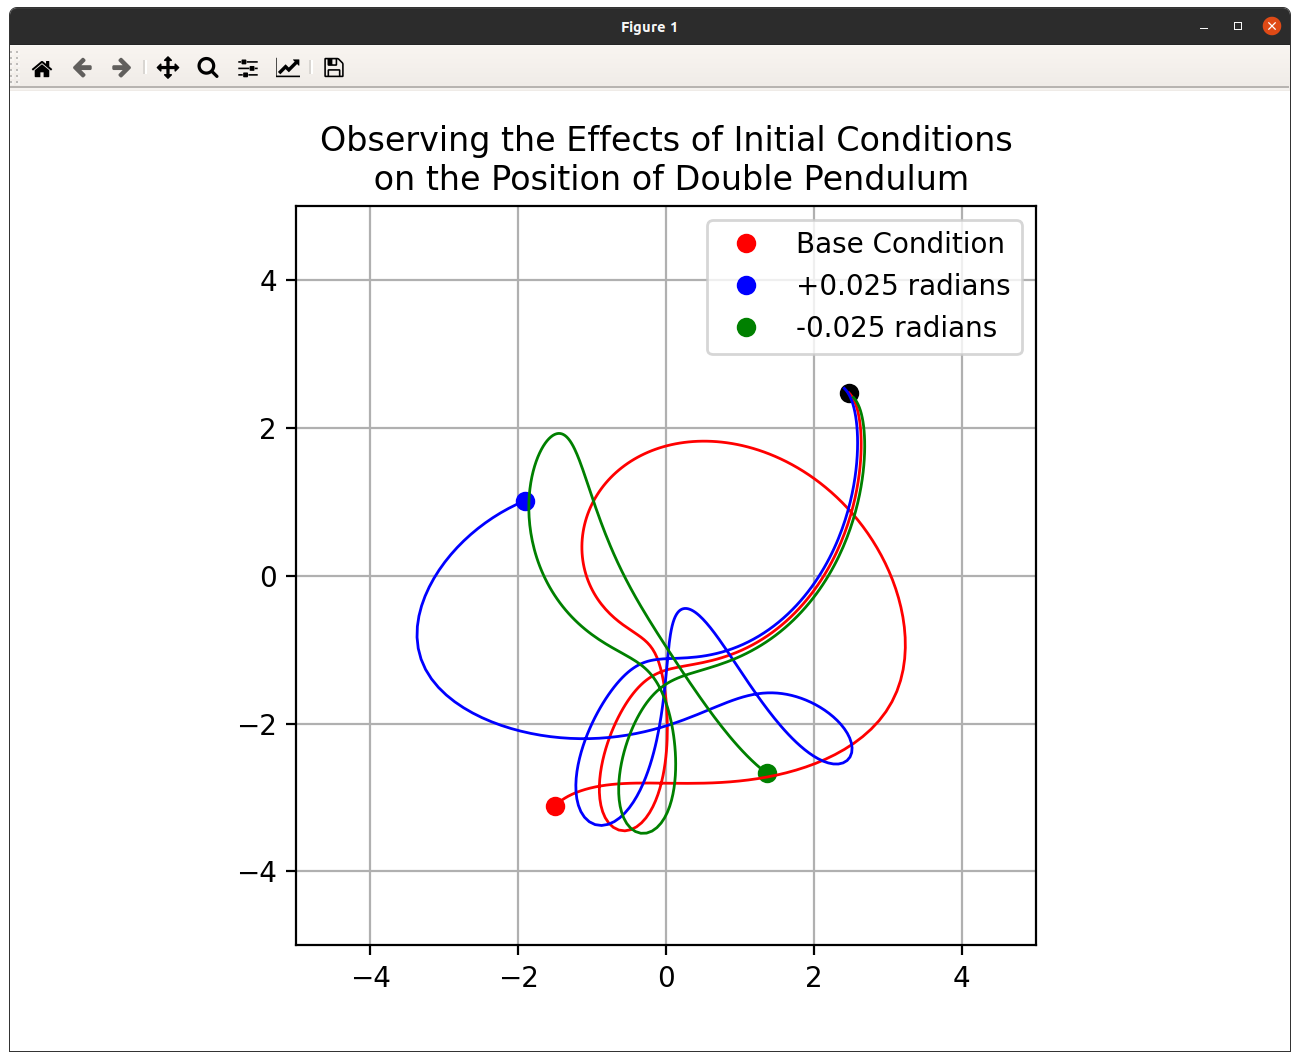
\includegraphics[scale=0.18]{chaos1.png}
    \captionof{figure}{Starting to diverge}
    \label{fig:chaos1}
  \end{minipage}%
  \begin{minipage}{.5\textwidth}
    \centering
    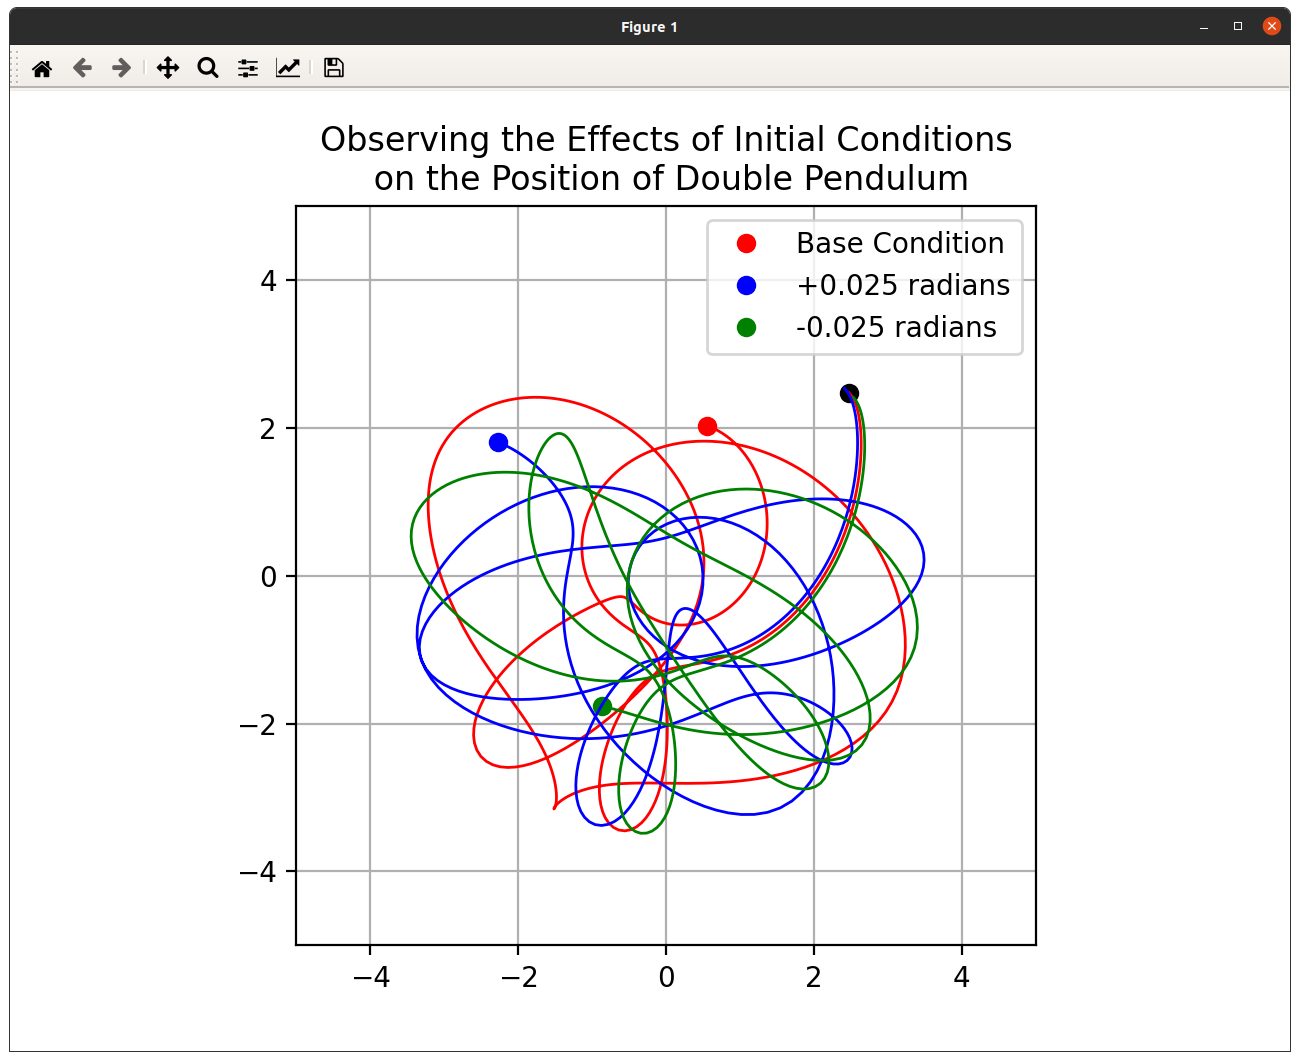
\includegraphics[scale=0.18]{chaos2.png}
    \captionof{figure}{Completely chaotic}
    \label{fig:chaos2}
  \end{minipage}
  \end{figure}

\begin{Example}
  The standard tent map $T(u)=1-|2u-1|$ defined on $[0,1]$ is a common example of a dynamical system satisfying these three properties. 
  \begin{figure}
    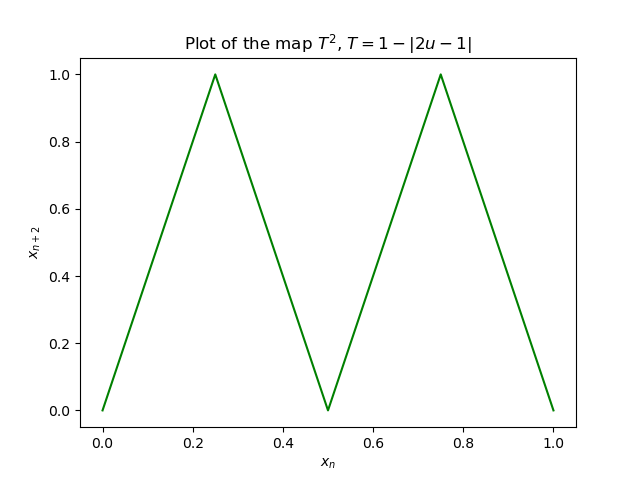
\includegraphics[scale=0.6]{T2.png}
    \centering
    \label{fig:T2tentmap}
  \end{figure}

  Let us now consider why this map exhibit's Devaneys's sense of chaos. The graph of the map $T$ is piecewise linear with two straight lines, one connecting the points $(0,0)$ and $(1/2,1)$ and the other connecting $(1/2,1)$ with $(1,0)$. They form a so-called tent with base centered at $u=1/2$. The graph of the map $T^2$ comprises two symmetric tents with their base centered at $1/4$ and $3/4$.
  % We now reason as why this map exhibits chaos in the sense of Devaney.   
  
  Given any point $u$ and an open neighborhood $W \subset[0,1]$ of $u$, we can find $k\in\mathbb{Z}$ large enough so that $T^k(W) = [0,1]$ because we can accommodate a tent whose base is contained in $W$. \emph{This last phrase doesn't make sense to me.} This implies the existence of two points $w_1$ and $w_2$ in $W$ so that $d(T^kw_1,T^kw_2)= 1$, and by the triangle inequality  at least one of the inequalities $d(T^ku,T^kw_1)> \delta$ or $d(T^ku,T^kw_2)> \delta$ hold when $\delta\in (0,1/2)$. \newline So $T$ has sensitive dependence on initial conditions.  
  
  Next, let $W_1$ and $W_2$ be two nonempty open sets. Given any open set $W_1$, we can find a $k\in\mathbb{N}$ large enough so that $T^k(W_1) = [0,1]$ because we can accommodate a tent with base contained in $W$. So $T^k(W_1) \cap W_2 \not=\emptyset$, and thus $T$ has topological transitivity.
  
  Finally, for every open interval $(a,b)$, the graph of $T^k$ intersects the graph of the identity map on $[0,1]$. This follows from the fact established above that there exists a $k\in\mathbb{N}$ such that $T^k(a,b) = [0,1]$.If the intersection point has coordinates of the form $(p,p)$, the point p is then a fixed point of $T^k$ and therefore also a periodic point of T. It follows that the set of periodic points are dense in T.
  \textbf{Expand further on reason for density.}
\end{Example}





\subsection{Conjugacy}

We now turn our attention to the subject of conjugacy. 

To show topological similarity or sameness between two metric or topological spaces, one needs to establish a homeomorphism between the two spaces. 
However, in the study of dynamical systems defined on two spaces, establishing a homeomorphism does not indicate that the systems are (physically) related in any way. \textbf{"related" - in what sense am I saying it here? Physically?}  For this one rather needs to establish a kind of dynamical equivalence which we illustrate in a simple commutativity diagram below.
% Giving errors
\begin{equation}  \label{eqn_conjugacy}
%    \[ 
    \psset{arrows=->, arrowinset=0.25, linewidth=0.6pt, nodesep=3pt, labelsep=2pt, rowsep=0.7cm, colsep = 1.1cm, shortput =tablr}
 \everypsbox{\scriptstyle}
 \begin{psmatrix}
U & U\\%
V & V.
 %%%
%  \ncline{1,1}{1,2}^{T} 
%  \ncline{1,1}{2,1} <{\phi}
%   \ncline{2,1}{2,2}^{S}
%  \ncline{1,2}{2,2} > {\phi}
 \end{psmatrix}
% \]
\end{equation} 
To understand the diagram we note that if we travel ``right and then down," the diagram instructs us to use $T$ (top arrow right) first, followed by $\phi$. (right arrow downwards). As a result, the pathway amounts to finding $\phi(T(u))$. If we proceed ``down and then right," the diagram instructs us to apply $\phi$ (left arrow downwards) first, and then apply $\phi$ (right arrow downwards) and then $S$ (bottom arrow right). As a result, the pathway amounts to finding  $S(\phi(u))$. When the diagram holds, we say 
$\phi(T(u))= S(\phi(u))$ and write it more formally as
$\phi \circ T=S\circ \phi$.
When the above commutativity holds in addition that $\phi$ is a homeomorphism, then we say we say that  $S$ is conjugate to $T$.  
If we relax the criterion on $\phi$ to merely require $\phi$ to be continuous and surjective rather than being a homeomorphism, then $\phi$ is called a semi-conjugacy, and declare that $S$ is semi-conjugate to $T$. When $S$ is conjugate to $T$, it indicates the dynamics between the two systems are in one-to-one correspondence, however when $S$ is semi-conjugate to $T$ with $\phi$ a many-to-one mapping, the dynamics on $V$ provides a coarse-grained description of the dynamics on $V$. It is common to remark that $S$ is a factor of $T$ or that $T$ is an extension of $S$ when $S$ is semi-conjugate to $T$. In essence, an extension (e.g., \cite{de2013elements}) is a larger system that captures all of the important dynamics of its factor.

It is a very hard or nearly an impossible task to establish the existence of a conjugacy or a semi-conjugacy $\phi$ between two systems. However, one can verify if given a function $\phi$ if it satisfies the commutativity.  For example $\phi(x)=\sin(\pi x/2)^2$ is a conjugacy between two systems $Tu=1-|2u-1|$ and $Sv=4v(1-v)$  defined on $[0,1]$.  The importance of conjugacy is that when we know it exists we can prefer to work with  the dynamical systems to gain information of the other, and this is useful for us while forecasting dynamical systems.  






\vspace{-1cm}
\bibliographystyle{pnas-new}
\bibliography{pnas}


\end{document}
